% Copyright 2004 by Till Tantau <tantau@users.sourceforge.net>.
%
% In principle, this file can be redistributed and/or modified under
% the terms of the GNU Public License, version 2.
%
% However, this file is supposed to be a template to be modified
% for your own needs. For this reason, if you use this file as a
% template and not specifically distribute it as part of a another
% package/program, I grant the extra permission to freely copy and
% modify this file as you see fit and even to delete this copyright
% notice. 

\documentclass{beamer}

\usepackage{blindtext}
\usepackage{tcolorbox}
\usepackage{soul}

\usepackage{amsmath}

\makeatletter
\newcommand\xleftrightarrow[2][]{%
  \ext@arrow 9999{\longleftrightarrowfill@}{#1}{#2}}
\newcommand\longleftrightarrowfill@{%
  \arrowfill@\leftarrow\relbar\rightarrow}
\makeatother

\usefonttheme{professionalfonts} % using non standard fonts for beamer
\usefonttheme{serif} % default family is serif
%\usepackage{fontspec}
%\setmainfont{Liberation Serif}

% There are many different themes available for Beamer. A comprehensive
% list with examples is given here:
% http://deic.uab.es/~iblanes/beamer_gallery/index_by_theme.html
% You can uncomment the themes below if you would like to use a different
% one:
%\usetheme{AnnArbor}
%\usetheme{Antibes}
%\usetheme{Bergen}
%\usetheme{Berkeley}
%\usetheme{Berlin}
%\usetheme{Boadilla}
%\usetheme{boxes}
%\usetheme{CambridgeUS}
%\usetheme{Copenhagen}
%\usetheme{Darmstadt}
\usetheme{default}
%\usetheme{Frankfurt}
%\usetheme{Goettingen}
%\usetheme{Hannover}
%\usetheme{Ilmenau}
%\usetheme{JuanLesPins}
%\usetheme{Luebeck}
%\usetheme{Madrid}
%\usetheme{Malmoe}
%\usetheme{Marburg}
%\usetheme{Montpellier}
%\usetheme{PaloAlto}
%\usetheme{Pittsburgh}
%\usetheme{Rochester}
%\usetheme{Singapore}
%\usetheme{Szeged}
%\usetheme{Warsaw}



\title{Introduction to Signal Processing}

% A subtitle is optional and this may be deleted
\subtitle{Lecture 5: \textbf{Fourier Transform and its Properties}}

\author{Sivakumar Balasubramanian}
% - Give the names in the same order as the appear in the paper.
% - Use the \inst{?} command only if the authors have different
%   affiliation.

\institute[Christian Medical College] % (optional, but mostly needed)
{
  \inst{}%
  Department of Bioengineering\\
  Christian Medical College, Bagayam\\
  Vellore 632002
}
% - Use the \inst command only if there are several affiliations.
% - Keep it simple, no one is interested in your street address.

\date{}
% - Either use conference name or its abbreviation.
% - Not really informative to the audience, more for people (including
%   yourself) who are reading the slides online

\subject{Lecture notes on signal processing}
% This is only inserted into the PDF information catalog. Can be left
% out.

% If you have a file called "university-logo-filename.xxx", where xxx
% is a graphic format that can be processed by latex or pdflatex,
% resp., then you can add a logo as follows:

% \pgfdeclareimage[height=0.5cm]{university-logo}{university-logo-filename}
% \logo{\pgfuseimage{university-logo}}

% Delete this, if you do not want the table of contents to pop up at
% the beginning of each subsection:
\AtBeginSubsection[]
{
  \begin{frame}<beamer>{Outline}
    \tableofcontents[currentsection,currentsubsection]
  \end{frame}
}

% Let's get started
\begin{document}

\begin{frame}
  \titlepage
\end{frame}

% READING MATERIAL
\begin{frame}{Reading material}

\begin{itemize}
\item Continuous-time Fourier series and Fourier transform of Chapter 3 from [2].
\item Chapter 4 from [3].
\item \textbf{Extra reading material:} (Highly recommended) Sections 4.4.1-4.4.6, 4.5 from [5]. 
\end{itemize}

\end{frame}


% EIGENFUNCTION AND EIGEN VALUES
\begin{frame}{Eigenfunctions and Eigenvalues}

\begin{itemize}
\item Convolution integral provides everything one needs to know about the input-output relationship of a LTI system.
\[ y(t) = h(t) * x(t) = \int_{-\infty}^{\infty}h(\tau)x(t - \tau)d\tau \]
\item LTI systems have an interesting property, which comes across clearly through the convolution integral.
\vspace{2mm}

When $x(t) = e^{st}$, then
\[ y(t) = \int_{-\infty}^{\infty}h(\tau)x(t - \tau)d\tau = \int_{-\infty}^{\infty}h(\tau)e^{s(t - \tau)}d\tau \]
\[ y(t) = e^{st}\left(\int_{-\infty}^{\infty}h(\tau)e^{-s\tau}d\tau\right) \]
\end{itemize}

\end{frame}

% EIGENFUNCTION AND EIGEN VALUES
\begin{frame}{Eigenfunctions and Eigenvalues}

\begin{itemize}
\item The output of an LTI system to $e^{st}$ is simply the product of $e^{st}$ with scalar value $\lambda_s = \int_{-\infty}^{\infty}h(\tau)e^{-s\tau}d\tau$.

\item A function that satisfies this property called an \textbf{eigenfunction} of the system, i.e.
\[ y(t) = H\left\{x(t)\right\} = \lambda x\left(t\right) \]

where, $\lambda$ is the \textbf{eigenvalue} corresponding to the input $x(t)$.
\item Signals $e^{st}$ are eigenfunctions of LTI systems, and their eigenvalue is given by,
\[ H(s) \triangleq \int_{-\infty}^{\infty}h(\tau)e^{-s\tau}d\tau \]
\item The eigenvalue is obtained from the impulse response.
\end{itemize}
\end{frame}

% WHAT USE IS AN EIGENFUNCTION?
\begin{frame}{What use is an eigenfunction?}

\begin{itemize}
\item Eigenfunctions help replace the convolution operation to a multiplication process.

\item If any signal $x(t)$ can be represented as a linear combination of eigenfunctions, then the output is the superposition of the scaled eigenfunctions.

\[ x(t) = \sum_{i=0}^{N-1} a_ie^{s_{i}t} \mapsto y(t) = \sum_{i=0}^{N-1} a_iH(s_i)e^{s_{i}t} \]

where, 
\[ H(s) = \int_{-\infty}^{\infty}h(t)e^{-st}dt \]

\item When $s=j\omega$, then we get the \textbf{Fourier transform} of a signal $h(t)$.
\[ H(\omega) \triangleq \int_{-\infty}^{\infty}h(t)e^{-j\omega t}dt \]
\end{itemize}
\end{frame}

% FOURIER TRANSFORM
\begin{frame}{Fourier Transform}

\textbf{Definition:}

The \textit{Fourier transform} of a signal $x(t)$ is defined as,
\[ X(\omega) = \int_{-\infty}^{\infty}x(t)e^{-j\omega t}dt \]

$X(\omega)$ exists if the above integral converges for all $\omega \in \mathbb{R}$. The \textit{inverse Fourier transform} is given by,
\[ x(t) = \frac{1}{2\pi}\int_{-\infty}^{\infty}X(\omega)e^{j\omega t}d\omega \]

$x\left(t\right)$ exists if the above integral converges for all $t \in \mathbb{R}$.

When both these exists, they are called the \textit{Fourier transform pairs},
\[ x(t) \xleftrightarrow{\text{FT}} X(\omega) \]

\end{frame}

% FOURIER TRANSFORM
\begin{frame}{Fourier transform}

\begin{itemize}
\item The Fourier transform definition is formally equivalent to the inner-product of finite energy signals (i.e. signals in $\mathcal{L}^2\left(\mathbb{R}\right)$)

\[ X(\omega) = \int_{-\infty}^{\infty}x(t)e^{-j\omega t}dt \]

\textbf{Note:} $e^{j\omega t}$ is not in $\mathcal{L}^2\left(\mathbb{R}\right)$.

\item Given that the Fourier transform and its inverse look very similar, the conditions for their existence are identical.

\item For most practical signals we will encounter, we will not have to worry about the technical details of the existence of the Fourier transform and its inverse.
\end{itemize}

\end{frame}

% EXISTENCE OF FOURIER TRANSFORM
\begin{frame}{Existence of Fourier transform\footnote{This slide can be skipped}}

\begin{itemize}
\item When a signal $x(t)$ is absolutely integrable, i.e. $x(t) \in \mathcal{L}^{1}\left(\mathbb{R}\right)$, then the Fourier transform $X(\omega)$ exists, and it is finite and continuous. 

\textit{You can understand this by analysing the following signal using the Fourier transform.}
\[ x(t) = \begin{cases}
\frac{1}{\sqrt{T}} & \left|t\right| \leq \frac{T}{2} \\
0 & \text{Otherwise}
\end{cases} \]

\textit{Is} $X(\omega)$ \textit{in} $\mathcal{L}^1\left(\mathbb{R}\right)$ \textit{?}

\item Fourier transforms can exist even when a signal is not in $\mathcal{L}^1\left(\mathbb{R}\right)$.

\item Fourier transforms can be used even when a signal does not have finite energy and is not absolutely integrable, such as the Dirac delta function.

\end{itemize}

\end{frame}

% PROPERTIES OF FOURIER TRANSFORM
\begin{frame}{Properties of Fourier transform}

Here are some of the basic properties of Fourier transform. It is left as an exercise to prove these for yourself.

\begin{itemize}
\item \textbf{Linearity}: $\alpha x(t) + \beta y(t) \xleftrightarrow{\text{FT}} \alpha X(\omega) + \beta Y(\omega)$
\item \textbf{Shift in time}: $ x(t-t_0) \xleftrightarrow{\text{FT}} e^{-j\omega t_0}X(\omega)$
\item \textbf{Shift in frequency}: $ x(t)e^{j\omega_0 t} \xleftrightarrow{\text{FT}} X(\omega - \omega_0) $
\item \textbf{Time and frequency scaling}: $ x(\alpha t) \xleftrightarrow{\text{FT}} \frac{1}{\alpha} X\left(\frac{\omega}{\alpha}\right), \,\, \alpha > 0 $
\item \textbf{Differentiation in time}: $\frac{d^nx(t)}{dt^n} \xleftrightarrow{\text{FT}} \left(j\omega\right)^nX(\omega)$
\item \textbf{Integration in time}: $\int_{-\infty}^{t}x(\tau)d\tau  \xleftrightarrow{\text{FT}} \frac{1}{j\omega}X(\omega); \, X(0) = 0$
\item \textbf{Convolution in time}: $x(t) * y(t) \xleftrightarrow{\text{FT}} X(\omega)Y(\omega) $
\item \textbf{Parseval's equality}: $\int_{-\infty}^{\infty}\left|x(t)\right|^2dt = \frac{1}{2\pi}\int_{-\infty}^{\infty}\left|X(\omega)\right|^2d\omega$
\end{itemize}

There are several other properties, which are left as an exercise for the student to explore.
\end{frame}

% SOME FOURIER TRANSFORM PAIRS
\begin{frame}{Some Fourier transform pairs}
\begin{itemize}
\item Rectangular pulse $x(t) = \begin{cases} 1 & \left|t\right| < 0.5 \\ 0 & \text{Otherwise} \end{cases}$
\begin{figure}
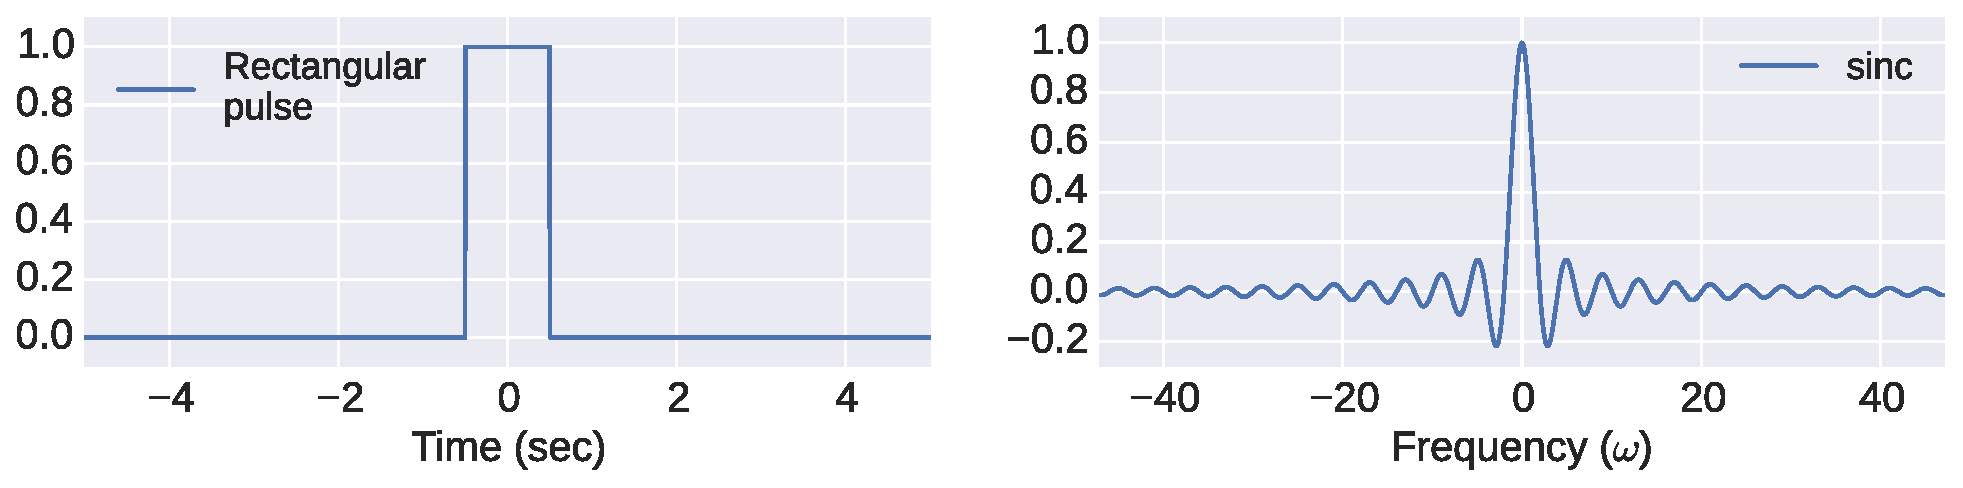
\includegraphics[width=\textwidth]{img/ft_rect_sinc.eps}
\end{figure}

\item Triangular pulse $x(t) = \begin{cases} 1 - \left|t\right| & \left|t\right| < 1 \\ 0 & \text{Otherwise} \end{cases}$
\begin{figure}
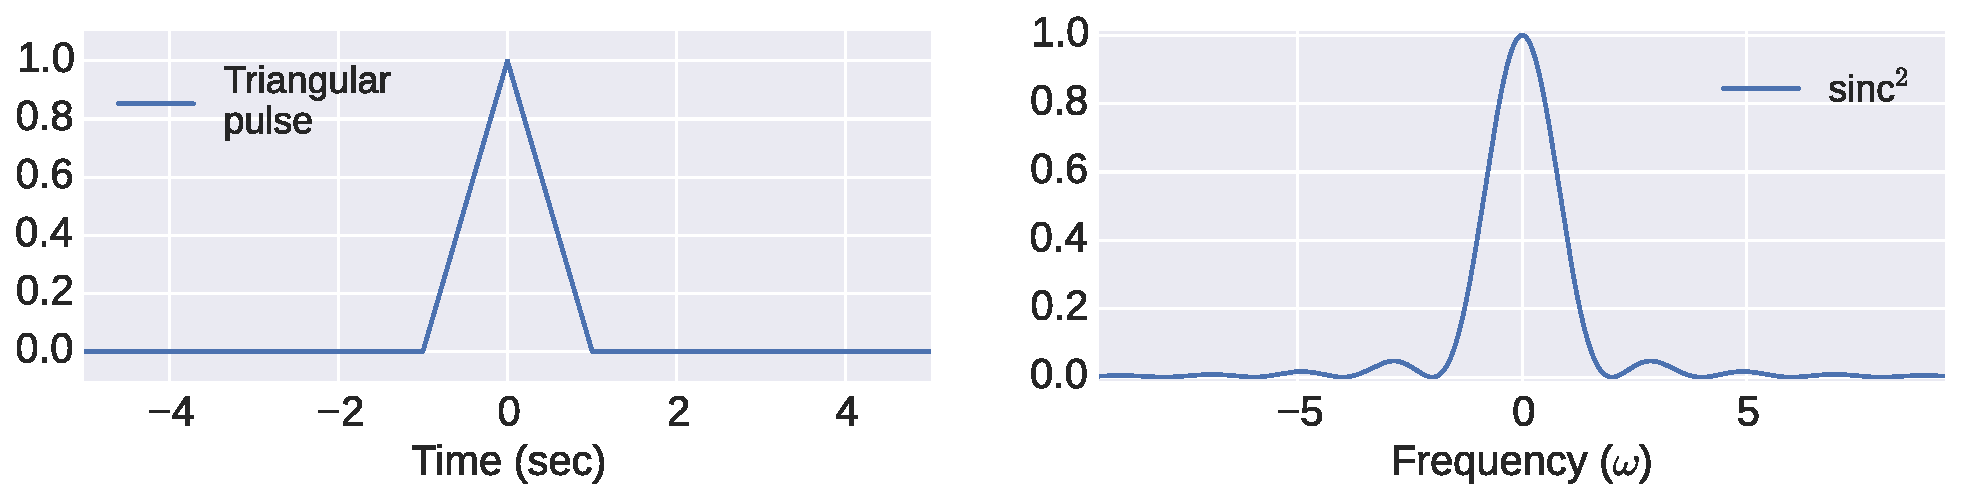
\includegraphics[width=\textwidth]{img/ft_tri_sinc2.eps}
\end{figure}
\end{itemize}

\end{frame}

% SOME FOURIER TRANSFORM PAIRS
\begin{frame}{Some Fourier transform pairs}
\begin{itemize}
\item DC signal, $x(t) = 1 \,\,\,\, \xleftrightarrow{FT} \,\,\,\, 2\pi \delta(\omega)$

\item Sinusoid, $x(t) = \sin \omega_0t \,\,\,\, \xleftrightarrow{FT} \,\,\,\, \pi \delta(\omega-\omega_0) + \pi \delta(\omega + \omega_0)$

\item Decaying exponential, $x(t) = e^{-\alpha t}u(t), \alpha > 0 \,\,\,\, \xleftrightarrow{FT} \,\,\,\, ?$

\item Unit step, $x(t) = u(t) \,\,\,\, \xleftrightarrow{FT} \,\,\,\, ? $

\item Gaussian signal, $x(t) = e^{-\alpha t^2}, \alpha > 0 \,\,\,\, \xleftrightarrow{FT} \,\,\,\, ? $

\end{itemize}

\end{frame}

% FREQUENCY RESPONSE
\begin{frame}{Frequency reseponse of LTI system}

\begin{itemize}
\item The Fourier transform allows the representation of any aperiodic signal as a scaled superposition of sinusoids, as long as the Fourier transform representation exists.

\item Once we know the Fourier representation of an input signal $x(t)$, we can use the eigenfunction property of a LTI system to estimate its output, i.e. scale each sinusoidal component (eigenfunction) by the appropriate eigenvalue and sum the scaled eigenfunctions to obtain the output.

\item But, how does one find out the eigenvalues of a LTI system? \textit{The impulse response}

\item The eigenvalues are given by the Fourier transform of impulse response, which is called the \textbf{frequency response} of the LTI system.
\[ H\left(\omega\right) = \int_{-\infty}^{\infty}h(t)e^{-j\omega t}dt \]

\end{itemize}

\end{frame}


% FREQUENCY RESPONSE
\begin{frame}{Frequency reseponse of LTI system}

\begin{itemize}
\item $H(\omega)$ is the eigenvalue for the eigenfunction $e^{j\omega t}$.
\item The output of the system to an input $x(t)$ is given by,
\[ y(t) = \int_{-\infty}^{\infty} X(\omega)H(\omega)e^{j\omega t} d\omega \]

Can you explain what is going on here? Also, try to relate the convolution property of the Fourier transform with the above relation.

\end{itemize}

\end{frame}

% FREQUENCY RESPONSE
\begin{frame}{Frequency reseponse of LTI system}

\begin{itemize}
\item $H(\omega)$ is a complex quantity with a real and imaginary part.
\[ H(\omega) = H_r(\omega) + jH_i(\omega) = \left|H(\omega)\right|e^{j\theta(\omega)}\]

where, $\left|H(\omega)\right|$ is the \textit{magnitude response}, and $\theta(\omega)$ is the \textit{phase response}.

\item The magnitude and phase response values are the amount of attenuation and the amount of phase shift introduced to an eigenfunction by an LTI system. i.e.

\[ e^{j\omega t} \mapsto \left|H(\omega)\right|e^{j\left(\omega t + \theta(\omega)\right)} \]

\item This implies that LTI system can be used for implementing \textit{frequency selective} filters, which manipulate the frequency content of any signal.
\end{itemize}

\end{frame}

% PROPERTIES OF FREQUENCY RESPONSE
\begin{frame}{Properties of frequency response}

Let $x(t) = x_r(t) + jx_i(t)$, and its Fourier transform is $X(\omega) = X_r(\omega) + jX_i(\omega).$
\vspace{2mm}

Fourier transforms have the following properties:
\begin{itemize}
\item $x(t) \text{ is real} \implies X(-\omega) = X^*(\omega) $
\item $x(t) \text{ is imaginary} \implies X(-\omega) = -X^*(\omega) $
\item $x(t) \text{ is even} \implies X(\omega) \text{ is real} $
\item $x(t) \text{ is odd} \implies X(\omega) \text{ is imaginary} $
\end{itemize}
\vspace{2mm}

When $x(t)$ is causal, such that $x(t) = 0, \,\, \forall t < 0$, then the real and imaginary components of the Fourier transform $X(\omega)$ are not independent of each other.
\vspace{2mm}

This implies that \textbf{one cannot have causal LTI system with arbitrary magnitude and phase responses}.

\end{frame}

% FOURIER SERIES
\begin{frame}{Fourier Series}

The Fourier series representation allows periodic signals to be represented as a sum of sinusoids.
\vspace{2mm}

\textbf{Definition}
The \textit{Fourier series} representation of a periodic signal $x(t)$ with fundamental period $T$, is given by
\[ x(t) = \sum_{k\in\mathbb{Z}}X_ke^{j(2\pi k/T)t}, \,\, t \in \left[\left.\frac{-T}{2}, \frac{T}{2}\right.\right) \]

where, $X_k$ is the \textit{Fourier series coefficient}
\[ X_k = \frac{1}{T}\int_{-T/2}^{T/2}x(t) e^{-j(2\pi k/T)t}dt, \,\, k \in \mathbb{Z} \]

$X_k$ exists if the above integral defined and finite for all  $k \in \mathbb{Z}$.

When $X_k$ exists, we have the \textit{Fourier series pair}
\[ x(t) \xleftrightarrow{FS} X_k \]

\end{frame}

% FOURIER SERIES
\begin{frame}{Fourier Series}

\begin{itemize}
\item The Fourier series coefficient is related to the Fourier transform. Consider a periodic signal $x(t)$, and its Fourier series coefficient $X_k$. 

Let us now consider a signal $\hat{x}(t)$, such that 
\[ \hat{x}(t) = x(t), t \in [-T/2, T/2) \]

In this case,
\[ X_k = \frac{1}{T}\hat{X}\left(\frac{2\pi}{T}k\right), \,\,\, k \in \mathbb{Z} \]
\end{itemize}

\end{frame}

% FOURIER SERIES
\begin{frame}{Existence of Fourier series\footnote{This slide can be skipped}}

\begin{itemize}
\item Existence of Fourier series coefficients are usually clearer than that of the Fourier transform, because the integral is over a finite interval.

\item When a function is absolutely integrable in one period, then the Fourier serious coefficients exist. Any continuous periodic function will have Fourier series coefficients.

\item Even when $X_k$ exists, we are still left with the question of how well we can recover $x(t)$ from the $X_k$s.
\vspace{2mm}

Consider $x(t)$, whose Fourier series coefficients are $X_k$. Now, considered the reconstructed signal, $\hat{x}(t)$:
\[ \hat{x}(t) = \sum_{k\in \mathbb{Z}} X_ke^{j(2\pi k/T)t} \]
\end{itemize}

\end{frame}

% FOURIER SERIES
\begin{frame}{Existence of Fourier series\footnote{This slide can be skipped}}

\begin{itemize}
\item The reconstructed signal equals the original signal for every time point, i.e.
\[ \hat{x}(t) = x(t), \,\,\, \forall t \in [-T/2, T/2), \iff \sum_{n\in\mathbb{Z}} \left|X_k\right| < \infty \]

\item When  $x(t)$ is finite but discontinuous, then we do not have pointwise equality. But the means squared error between $x(t)$ and $\hat{x}(t)$ is zero. $\int_{-T/2}^{T/2}\left|x(t) - \hat{x}(t)\right|^2dt = 0$

\item This can be understood with the following example. Determine the Fourier series coefficients for the following $x(t) = \begin{cases}
1 & t \in \left[-\frac{T}{4}, \frac{T}{4}\right] \\
0 & t \in \left[\left.-\frac{T}{2}, -\frac{T}{4}\right.\right) \\
0 & t \in \left(\frac{T}{4}, \frac{T}{2}\right)
\end{cases}$

What is value of the reconstructed signal $\hat{x}(t)$ at the discontinuities $t = \left\{-\frac{T}{4}, \frac{T}{4}\right\}$
\end{itemize}

\end{frame}

% PROPERTIES OF FOURIER SERIES
\begin{frame}{Properties of Fourier series}

The properties of the Fourier series are similar to that of the Fourier transform.

\begin{itemize}
\item \textbf{Linearity}: $\alpha x(t) + \beta y(t) \xleftrightarrow{\text{FT}} \alpha X_k + \beta Y_k$
\item \textbf{Shift in time}: $ x(t-t_0) \xleftrightarrow{\text{FT}} e^{-j(2\pi k/T)t_0}X_k$
\item \textbf{Shift in frequency}: $ x(t)e^{j(2\pi k_0/T)t} \xleftrightarrow{\text{FT}} X_{k-k_0} $
\end{itemize}

The other properties are left as an exercise for the student to explore.

\end{frame}

% FOURIER SERIES PAIRS
\begin{frame}{Fourier series pairs}

\begin{itemize}
\item Square wave, $x(t) = \begin{cases}
1 & t \in \left[-\frac{T}{4}, \frac{T}{4}\right] \\
0 & t \in \left[\left.-\frac{T}{2}, -\frac{T}{4}\right.\right) \\
0 & t \in \left(\frac{T}{4}, \frac{T}{2}\right)
\end{cases} \,\,\,\, \xleftrightarrow{FS} \,\,\,\, ?$
\item  Triangular wave, $x(t) = \frac{1}{2} - \left|t\right|, t \in \left[\left.\frac{-1}{2}, \frac{1}{2}\right.\right)  \,\,\,\, \xleftrightarrow{FS} \,\,\,\, ?$
\item  Dirac comb, $x(t) = s_{T}(t) = \sum_{n\in\mathbb{Z}} \delta\left(t - nT\right)  \,\,\,\, \xleftrightarrow{FS} \,\,\,\, ?$
\item  Sinusoid, $x(t) = \sin 0.75\pi t \,\,\,\, \xleftrightarrow{FS} \,\,\,\, ?$
\end{itemize}

\end{frame}

% RECONSTRUCTION OF SIGNALS FROM PARTIAL FOURIER COEFFICIENTS
\begin{frame}{Reconstruction of signals from finite number of Fourier coefficients}

\begin{itemize}
\item When a period signal is bounded, we know that the Fourier series coefficients will exist, and the reconstructed signal from the Fourier series coefficient will be equal to the original signal in the mean square sense. i.e,
\[ \int_{-T/2}^{T/2} \left|x(t) - \sum_{k\in\mathbb{Z}}X_ke^{j(2\pi k/T)t}\right|^2dt = 0 \]

\item What happens if we use only a finite number of Fourier series coefficients?, i.e.
\[ \hat{x}_N(t) = \sum_{k=-N}^{N}X_ke^{j(2\pi k/T)t} \]
\end{itemize}

\end{frame}

% RECONSTRUCTION OF SIGNALS FROM PARTIAL FOURIER COEFFICIENTS
\begin{frame}{Reconstruction of signals from finite number of Fourier coefficients}

Consider the following signal, $x(t) = \begin{cases}
1 & t \in [-0.25, 0.25] \\
0 & t \in [-0.5, -0.25) \\
0 & t \in (0.25, 0.5) \\
\end{cases}$

\begin{figure}
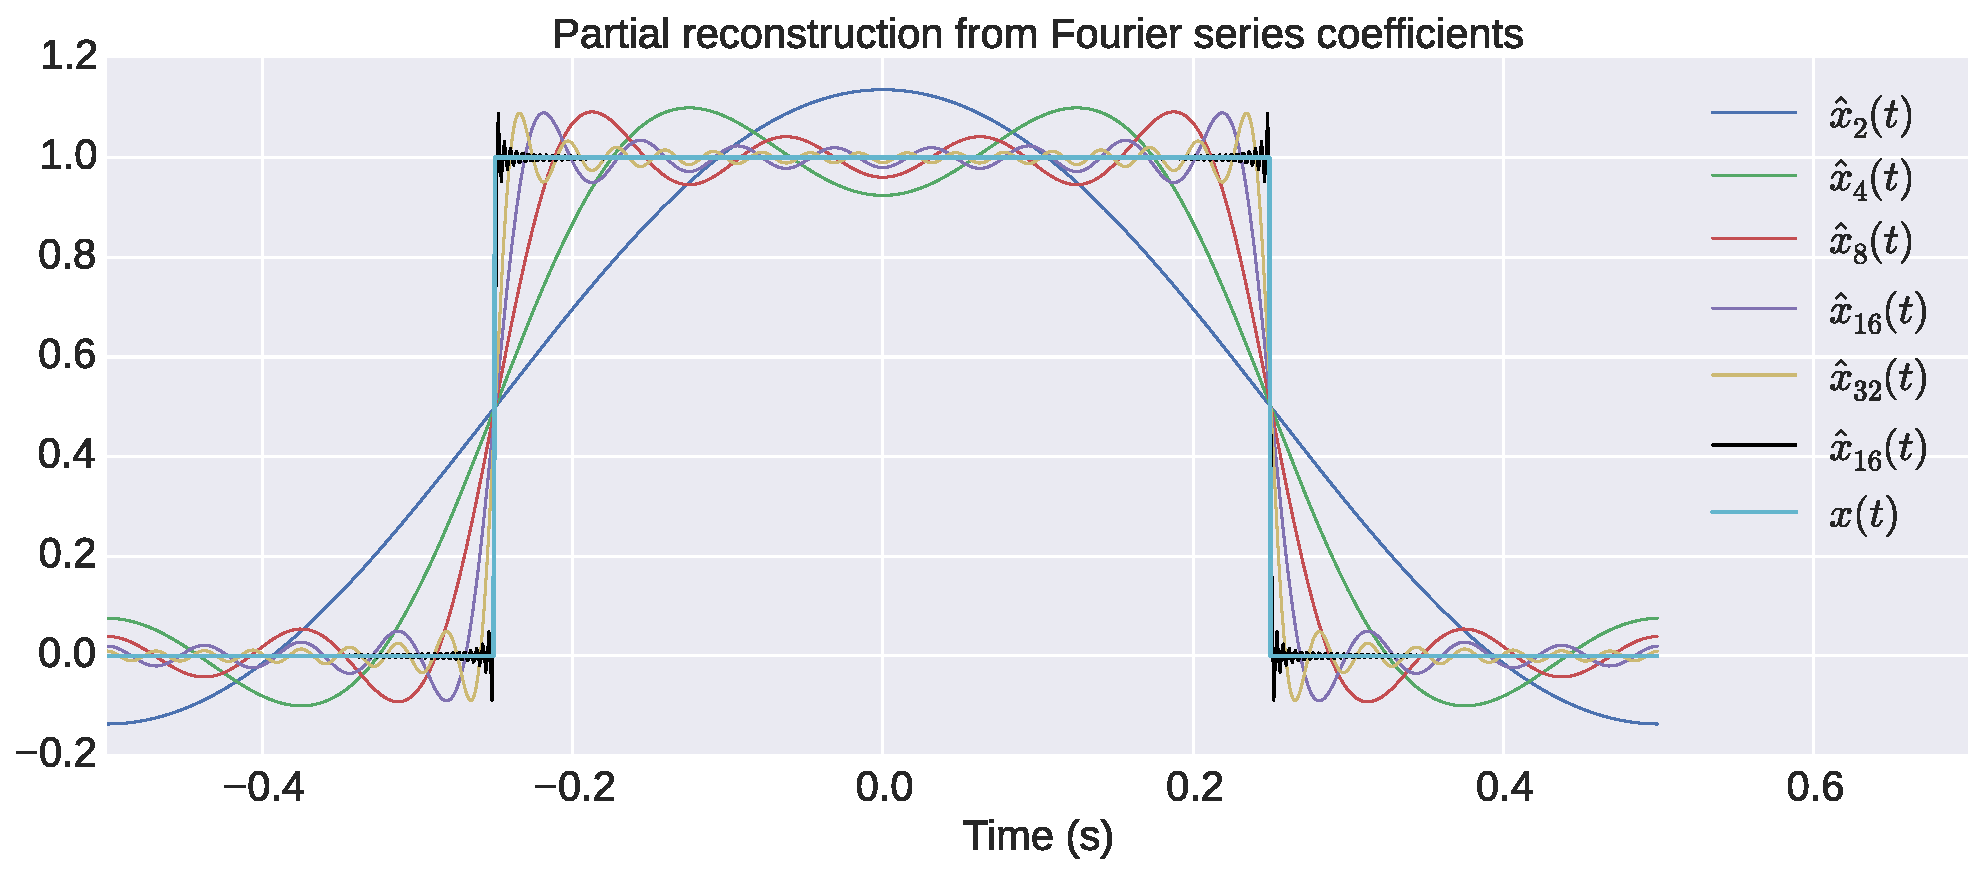
\includegraphics[width=\textwidth]{img/gibbs_fs.eps}
\end{figure}
\vspace{-5mm}

What all do you notice in the above partial reconstructions?

\end{frame}

% GIBBS PHENOMENON
\begin{frame}{Gibbs phenomenon}

\begin{figure}
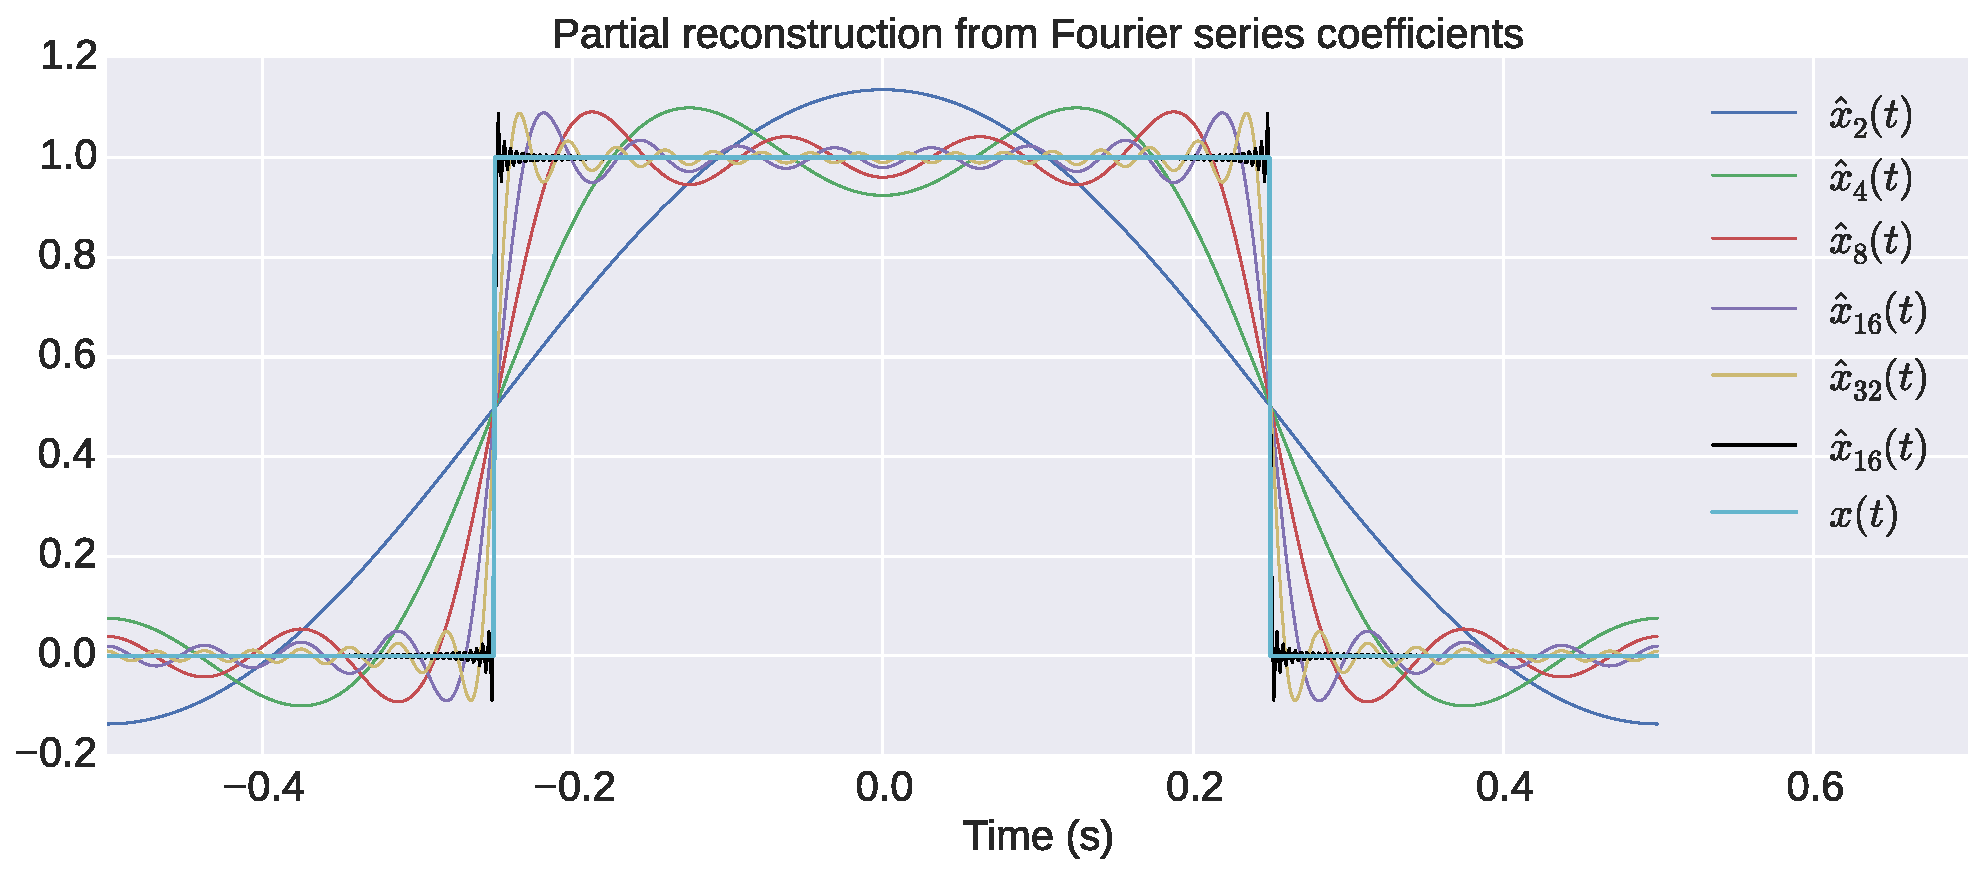
\includegraphics[width=\textwidth]{img/gibbs_fs.eps}
\end{figure}
\vspace{-5mm}

\begin{itemize}
\item As $N$ increases, $\hat{x}(t) \to x(t)$ everywhere, except at points close to the discontinuities.
\item $max_{t\in[-0.5, 0.5)}\left|x(t) - \hat{x}(t)\right|$ does not approach zero for any finite $N$.
\item This is the \textit{Gibbs phenomenon}. When $x(t)$ is discontinuous, we only have convergence in the mean squared sense, i.e. $\int_{-T/2}^{T/2} \left|x(t)-\hat{x}(t)\right|^2dt = 0$.
\end{itemize}

\end{frame}

% FOURIER TRANSFORM OF PERIODIC SIGNALS
\begin{frame}{Fourier transform of periodic signals}
\begin{itemize}
\item Periodic signals cannot have a Fourier transform in elementary sense, because periodic signals are not energy signals and they are not absolutely integrable. But using Dirac delta functions we can arrive at the Fourier transform on periodic signals.
\item Consider a time-limited signal, $\hat{x}(t)$ that is restricted to $t \in [-T/2, T/2)$. Let $\hat{X}(\omega)$ be its Fourier transform.
\item We can generate a periodic signal $x(t)$ from $\hat{x}(t)$, by the following,
\[ x(t) = \sum_{n\in\mathbb{Z}}\hat{x}(t - nT) = s_T(t) * \hat{x}(t) \]
Notice, that convolution between the Dirac delta comb and $\hat{x}(t)$ generates the periodic signal.
\end{itemize}
\end{frame}

% FOURIER TRANSFORM OF PERIODIC SIGNALS
\begin{frame}{Fourier transform of periodic signals}

\[ x(t) = \sum_{n\in\mathbb{Z}}\hat{x}(t - nT) = s_T(t) * \hat{x}(t) \]

This implies that,
\[ X(\omega) = S_T(\omega)\hat{X}(\omega) \]

Here (verify this),
\[ S_T(\omega) = \sum_{n\in\mathbb{Z}}e^{-j\omega nT} = \frac{2\pi}{T}\sum_{k\in\mathbb{Z}}\delta\left(\omega - \frac{2\pi}{T}k\right) = \frac{2\pi}{T}s_{2\pi/T}\left(\omega\right) \]

\[ X(\omega) = \frac{2\pi}{T}\sum_{k\in\mathbb{Z}}\hat{X}\left(\frac{2\pi}{T}k\right)\delta\left(\omega - \frac{2\pi}{T}k\right) = 2\pi\sum_{k\in\mathbb{Z}}X_k\delta\left(\omega - \frac{2\pi}{T}k\right) \]

Fourier transform of a periodic signal of period $T$ is weighted Dirac comb with spacing $2\pi/T$.

\end{frame}

\end{document}